\documentclass{article}

\PassOptionsToPackage{numbers,sort&compress}{natbib}
\usepackage[preprint]{neurips_2021}

\usepackage[utf8]{inputenc}
\usepackage[T1]{fontenc}
\usepackage{hyperref}
\usepackage{url}
\usepackage{booktabs}
\usepackage{amsfonts}
\usepackage{nicefrac}
\usepackage{microtype}
\usepackage{xcolor}
\usepackage{graphicx}
\usepackage{subcaption}
\usepackage{multirow}
\usepackage{array}
\usepackage{float}
\usepackage{amsthm}
\usepackage{amsmath}
\usepackage{amssymb}
\usepackage{mathtools}
\usepackage{enumitem}
\usepackage{algorithm}
\usepackage{algpseudocode}

\title{ROWA: Domain Generalization by Seeking Recoverable Checkpoints}

\author{Anonymous Authors}

\newtheorem{theorem}{Theorem}
\newtheorem{proposition}{Proposition}
\newtheorem{lemma}{Lemma}
\newtheorem{corollary}{Corollary}
\newtheorem{definition}{Definition}
\newtheorem{assumption}{Assumption}
\newtheorem{remark}{Remark}

\newcommand{\RR}{\mathbb{R}}
\newcommand{\EE}{\mathbb{E}}
\newcommand{\tr}{\operatorname{tr}}
\newcommand{\argmin}{\operatorname*{arg\,min}}
\newcommand{\diag}{\operatorname{diag}}
\newcommand{\TBD}{\textbf{TBD}}
\newcommand{\etal}{\textit{et al.}}
\newcommand{\ie}{\textit{i.e.}}
\newcommand{\eg}{\textit{e.g.}}
\newcommand{\iid}{i.i.d.}
\newcommand{\ood}{OOD}
\newcommand{\iidcaps}{IID}
\newcommand{\rowa}{\textup{\textsc{ROWA}}}
\newcommand{\swad}{\textup{\textsc{SWAD}}}
\newcommand{\maiwa}{\textup{\textsc{MAIWA}}}
\newcommand{\cowa}{\textup{\textsc{COWA}}}

\begin{document}

\maketitle

\begin{abstract}
Single-run post-hoc methods are among the most attractive tools for domain generalization because they can be added to strong empirical risk minimization pipelines without retraining. The current reference point in this regime is \swad, which selects and averages dense checkpoints by seeking flat pooled minima. We argue that flatness is an indirect proxy for the real single-run domain generalization problem. A good checkpoint should not merely tolerate isotropic perturbations; it should support \emph{cross-domain recovery}: when one source domain is held out, a small update computed from the other source domains should immediately improve the held-out one. This principle leads to Recoverability-Oriented Weight Averaging (\rowa), a simple post-hoc method that scores checkpoints by leave-one-domain-out one-step transfer and averages a contiguous low-score window. We develop a theory for \rowa under explicit local assumptions. First, we show that the exact \rowa score upper-bounds the held-out transfer loss through a smoothness inequality. Second, we derive a closed-form first-order decomposition showing that \rowa rewards shared descent while penalizing domain-gradient covariance. Third, we prove a separation result: there exist checkpoints with identical pooled loss and pooled flatness statistics that any flatness-only selector treats as equivalent, while \rowa strictly distinguishes them by transfer quality. Finally, we justify dense checkpoint sampling and low-score window averaging under local regularity assumptions. We include a complete NeurIPS-style manuscript, rigorous proofs, analytical figures, a reproducible experimental protocol, and published baseline numbers from prior work; all new quantitative results for \rowa remain intentionally marked as \TBD{} pending execution.
\end{abstract}

\section{Introduction}

Domain generalization (DG) asks for a model that performs well on an unseen target environment using only labeled source environments at training time. In practice, the most successful DG methods are often the ones that users can actually deploy: they preserve a standard empirical risk minimization (ERM) pipeline, add little extra machinery, and remain easy to tune. In this sense, \swad{} \citep{cha2021wad} is a particularly important reference point. It is single-run, post-hoc, cheap, and effective. On the five standard DomainBed benchmarks with ResNet-50, \swad{} reports a mean accuracy of $66.9$, improving over ERM's $63.3$ and over the best prior competitor's $65.3$ in the same evaluation family \citep{cha2021wad}. Diverse Weight Averaging (DiWA) later showed that weight averaging can go higher, reaching up to $68.0$ when it is allowed to average across many models and training runs \citep{rame2022diwa}, but that setting is operationally heavier.

The central question of this paper is therefore narrow and practical:
\begin{quote}
Can a single training trajectory contain enough information to produce a post-hoc selector that is as simple as \swad{}, but more directly targeted to domain generalization than pooled flatness?
\end{quote}

Our answer is \rowa{}, Recoverability-Oriented Weight Averaging. The principle is simple:
\begin{quote}
    A checkpoint is domain-general if any one source domain is recoverable by a tiny update computed from the other source domains.
\end{quote}
At checkpoint $\theta_t$, \rowa{} temporarily holds out domain $i$, forms a virtual update using the other source domains, and measures whether the held-out domain improves. The score is the average transferred held-out loss, optionally plus a robustness gap term. The final model is obtained by averaging a contiguous low-score window, exactly in the spirit of \swad{} and stochastic weight averaging (SWA) \citep{izmailov2018swa}.

This shift from \emph{flatness} to \emph{recoverability} matters because DG is not merely a problem of robustness to weight perturbations. A target domain is not an arbitrary perturbation in parameter space. It is a new environment that should be reachable from shared knowledge. Meta-learning methods already exploit this intuition during training, notably MLDG's one-step meta-train/meta-test objective \citep{li2018mldg} and first-order transfer analyses such as Reptile \citep{nichol2018reptile}. More recent DG work also moves toward one-step transfer signals during training. What is missing is a \emph{single-run post-hoc selector} that imports the same principle into the checkpoint-selection regime where \swad{} became influential.

We make four contributions.
\begin{enumerate}[leftmargin=1.4em]
    \item We introduce \rowa{}, a simple post-hoc DG algorithm that scores checkpoints by leave-one-domain-out one-step transfer and averages a contiguous low-score window.
    \item We prove a smoothness-based upper bound on the exact \rowa{} score and derive a closed-form decomposition showing that \rowa{} rewards shared descent while penalizing domain-gradient covariance.
    \item We prove a constructive separation theorem showing that pooled-flatness selectors can be blind to transfer-relevant differences that \rowa{} captures.
    \item We provide a complete publication-style paper draft with algorithms, proofs, analytical figures, experimental protocol, and prior published baselines; all new \rowa{} results remain explicitly marked \TBD{} because they have not been run yet.
\end{enumerate}

\begin{remark}
This paper does \emph{not} claim an unconditional theorem that \rowa{} empirically dominates \swad{} or every other DG method on all tasks. Such a theorem would be indefensible. Our theory instead proves that \rowa{} targets a different object, that this object is DG-relevant under explicit assumptions, and that flatness-only selectors provably miss it on a nontrivial class of examples.
\end{remark}

\begin{figure}[t]
    \centering
    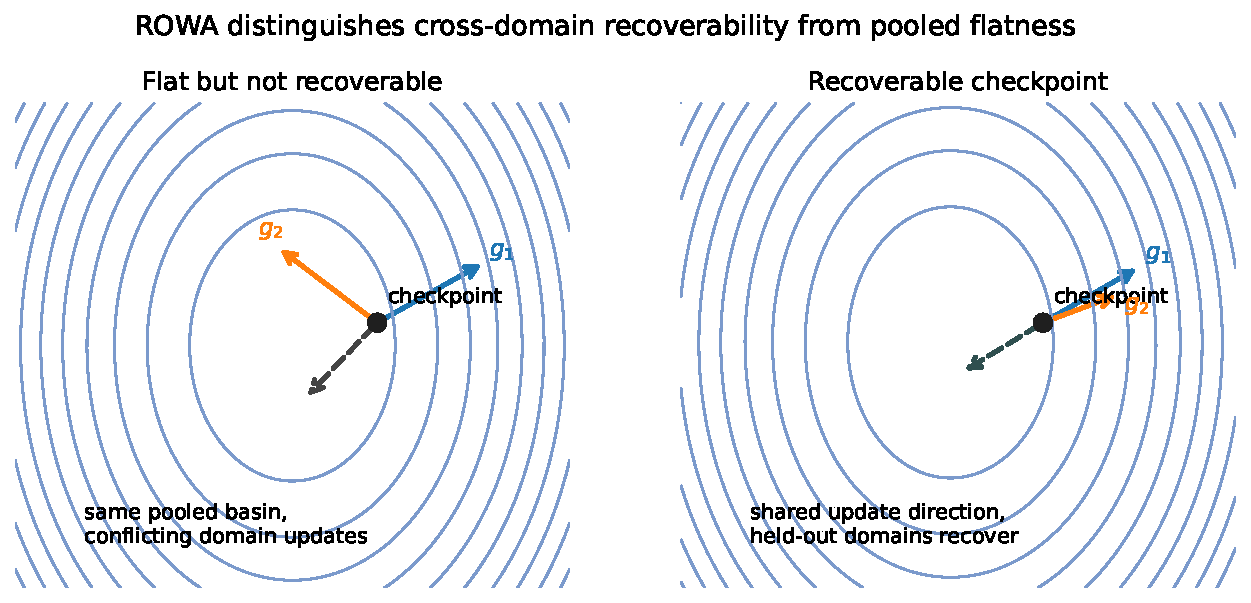
\includegraphics[width=\linewidth]{figures/geometry_recoverability_vs_flatness.pdf}
    \caption{\textbf{Conceptual geometry.} Two checkpoints can live in similarly flat pooled basins yet have very different cross-domain recoverability. \rowa{} asks whether a held-out domain improves after a tiny update from the other domains, which is a more direct DG probe than pooled flatness alone.}
    \label{fig:geometry}
\end{figure}

\section{Related Work}

\paragraph{Single-run post-hoc DG.}
\swad{} \citep{cha2021wad} is the canonical single-run post-hoc DG method. It connects flat minima to DG through robust empirical risk and proposes dense checkpointing with an overfit-aware start/end rule. Its practical appeal is precisely the appeal we want to preserve: one training run, no extra end-to-end optimization, and a final weight average. DiWA \citep{rame2022diwa} shows that more diverse model averaging can improve \ood{} performance further, but its strongest results rely on averaging across many models or runs. \rowa{} stays in the \swad{} regime and changes the selection principle rather than the computational regime.

\paragraph{Weight averaging and flatness.}
SWA \citep{izmailov2018swa} and mode-connectivity work \citep{garipov2018fge} established that averaging along a trajectory can find wider optima. This line has been highly influential, and \swad{} imports it into DG. But flatness only describes sensitivity to perturbations around a pooled objective. DG additionally depends on whether information from one environment helps another. Our theory below shows that \rowa{} isolates this missing cross-domain interaction term explicitly.

\paragraph{Meta-learning and one-step transfer.}
MLDG \citep{li2018mldg} optimizes a leave-one-domain-out objective during training by taking one gradient step on meta-train domains and evaluating on meta-test domains. Reptile \citep{nichol2018reptile} showed that first-order meta-learning updates are governed by gradient inner products across minibatches. More recent DG work continues to explore one-step generalization signals during training. \rowa{} differs in one crucial respect: it is not a training algorithm. It is a post-hoc checkpoint selector that extracts a one-step transfer signal from an ordinary trajectory.

\paragraph{Invariant and geometry-aware DG.}
Methods such as CORAL \citep{sun2016coral} and other invariant-feature or invariant-gradient approaches try to align geometry or training dynamics across domains. \rowa{} is compatible with these methods but orthogonal to them: it can be applied on top of any single trajectory, and its score directly tests whether cross-domain information improves a held-out domain.

\section{Recoverability-Oriented Weight Averaging}
\label{sec:method}

Assume source domains $\mathcal{E}_{1},\dots,\mathcal{E}_{I}$ and a single training run that produces checkpoints $\{\theta_t\}_{t=1}^{K}$. For each source domain $i$, we reserve a held-out split $V_i$ and define the held-out loss
\begin{equation}
    L_i(\theta) \triangleq \frac{1}{|V_i|}\sum_{(x,y)\in V_i} \ell(f_\theta(x), y).
\end{equation}
Let $g_{i,t} \triangleq \nabla_\theta L_i(\theta_t)$ denote the domain-wise gradient at checkpoint $t$ and define the leave-one-domain-out gradient
\begin{equation}
    g_{-i,t} \triangleq \nabla_\theta \frac{1}{I-1}\sum_{j\neq i} L_j(\theta_t)
    = \frac{1}{I-1}\sum_{j\neq i} g_{j,t}.
\end{equation}

We allow an optional positive semidefinite preconditioner $P_t \succeq 0$; the simplest choice is $P_t = I$. The virtual cross-domain update for held-out domain $i$ is
\begin{equation}
    \theta_{-i \rightarrow i,t}(\eta) \triangleq \theta_t - \eta P_t g_{-i,t},
\end{equation}
where $\eta > 0$ is a small transfer step size.

\subsection{Exact and first-order scores}

The exact \rowa{} core score is the average transferred held-out loss:
\begin{equation}
    R_t^{\mathrm{ex}}(\eta) \triangleq \frac{1}{I}\sum_{i=1}^{I}
    L_i\!\left(\theta_t - \eta P_t g_{-i,t}\right).
    \label{eq:exact_score}
\end{equation}
We optionally add a robustness gap penalty
\begin{equation}
    \mathrm{Gap}_t \triangleq \sqrt{\frac{1}{I}\sum_{i=1}^{I}\left(
    L_i\!\left(\theta_t - \eta P_t g_{-i,t}\right) - R_t^{\mathrm{ex}}(\eta)
    \right)^2},
\end{equation}
and define the practical score
\begin{equation}
    S_t^{\mathrm{ex}}(\eta,\lambda) \triangleq R_t^{\mathrm{ex}}(\eta) + \lambda\, \mathrm{Gap}_t.
\end{equation}

The cheap first-order variant linearizes the transferred loss:
\begin{equation}
    R_t^{\mathrm{fo}}(\eta) \triangleq
    \frac{1}{I}\sum_{i=1}^{I} \left(
        L_i(\theta_t) - \eta \langle g_{i,t}, P_t g_{-i,t}\rangle
    \right),
    \label{eq:first_order_score}
\end{equation}
and again adds the same or an analogous gap term.

\subsection{Checkpoint selection and window averaging}

Let $S_t$ denote either $S_t^{\mathrm{ex}}$ or $S_t^{\mathrm{fo}}$. We select
\begin{equation}
    t^\star \in \argmin_{1 \le t \le K} S_t
\end{equation}
and form a contiguous low-score window
\begin{equation}
    W_\delta \triangleq \{t: S_t \le S_{t^\star} + \delta\},
\end{equation}
restricted to the connected component of $t^\star$ if there are multiple disjoint sublevel intervals. The final model is the weight average
\begin{equation}
    \bar \theta_{\rowa} \triangleq \sum_{t \in W_\delta} w_t \theta_t,
    \qquad
    w_t \ge 0,\quad \sum_{t \in W_\delta} w_t = 1.
\end{equation}
Uniform weights are the default; softmin weights on $S_t$ are a valid variant.

\begin{figure*}[t]
    \centering
    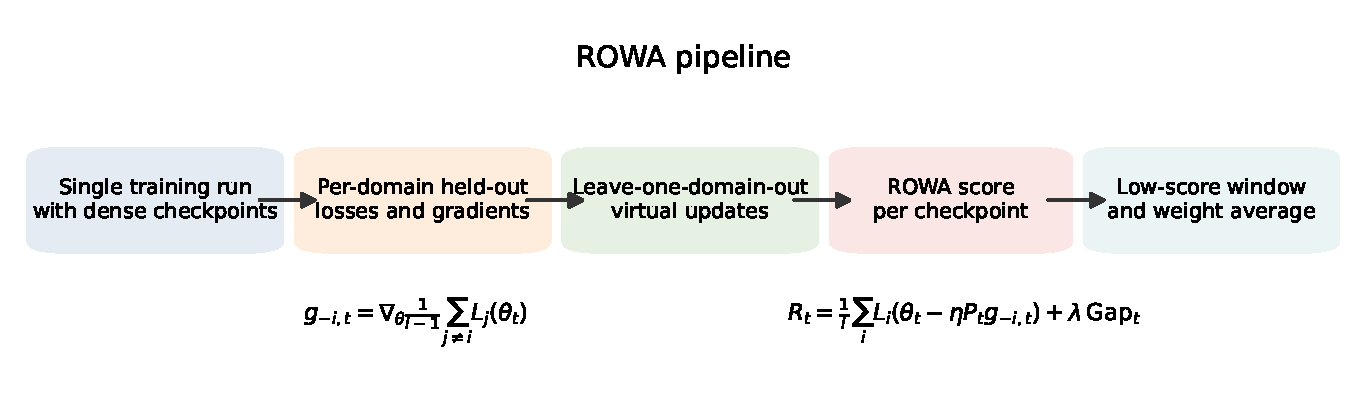
\includegraphics[width=0.95\textwidth]{figures/rowa_pipeline.pdf}
    \caption{\textbf{\rowa{} pipeline.} Starting from a single ordinary training run, \rowa{} uses per-domain held-out gradients to evaluate leave-one-domain-out virtual steps, scores every checkpoint by transfer quality, and averages a contiguous low-score window.}
    \label{fig:pipeline}
\end{figure*}

\begin{algorithm}[t]
    \caption{\rowa{} (\textsc{Recoverability-Oriented Weight Averaging})}
    \label{alg:rowa}
    \begin{algorithmic}[1]
        \Require Checkpoints $\{\theta_t\}_{t=1}^{K}$ from one training run; held-out source splits $\{V_i\}_{i=1}^{I}$; transfer step $\eta$; gap weight $\lambda$; sublevel width $\delta$; preconditioners $\{P_t\}_{t=1}^{K}$
        \For{$t=1,\dots,K$}
            \For{$i=1,\dots,I$}
                \State Compute $L_i(\theta_t)$ and $g_{i,t} = \nabla_\theta L_i(\theta_t)$ on $V_i$
            \EndFor
            \For{$i=1,\dots,I$}
                \State $g_{-i,t} \gets \frac{1}{I-1}\sum_{j \neq i} g_{j,t}$
                \State $u_{i,t} \gets L_i(\theta_t - \eta P_t g_{-i,t})$ \Comment{or first-order approximation}
            \EndFor
            \State $S_t \gets \frac{1}{I}\sum_i u_{i,t} + \lambda \cdot \mathrm{Gap}(u_{1,t},\dots,u_{I,t})$
        \EndFor
        \State $t^\star \gets \argmin_t S_t$
        \State $W_\delta \gets$ connected sublevel window around $t^\star$ satisfying $S_t \le S_{t^\star}+\delta$
        \State \Return $\bar \theta_{\rowa} = \sum_{t \in W_\delta} w_t \theta_t$
    \end{algorithmic}
\end{algorithm}

\paragraph{Practical complexity.}
The exact variant adds $I$ held-out gradients and $I$ held-out forward evaluations per checkpoint. The first-order variant removes the second set of forward passes. Since DomainBed benchmarks use small numbers of domains (typically four and at most six), the added cost is linear in a small constant and remains in the same operational regime as dense checkpoint selection.

\section{Theory}
\label{sec:theory}

We now analyze the \rowa{} core score. Throughout the theory section, we omit the optional gap penalty because it is nonnegative and orthogonal to the transfer mechanism. The theory below therefore targets the core quantity in Eq.~\eqref{eq:exact_score} and its first-order surrogate Eq.~\eqref{eq:first_order_score}.

\subsection{Population object}

\begin{definition}[Population recoverability risk]
Let $\rho$ be a distribution over environments. For a parameter vector $\theta$, transfer step $\eta$, and preconditioner $P$, define
\begin{equation}
    \mathcal{R}_{\rho}(\theta;\eta,P) \triangleq
    \EE_{E_0,E_1,\dots,E_{I-1}\sim \rho}
    \left[
    L_{E_0}\left(
    \theta - \eta P \frac{1}{I-1}\sum_{j=1}^{I-1}\nabla L_{E_j}(\theta)
    \right)
    \right].
\end{equation}
\end{definition}

This is the object \rowa{} tries to estimate. It asks exactly the DG-relevant question: if one fresh environment is held out and the others are used to produce a tiny update, how good is the result on the held-out environment?

\begin{proposition}[Exchangeable source environments make \rowa{} unbiased]
\label{prop:unbiased}
Suppose $E_1,\dots,E_I \stackrel{\iid}{\sim} \rho$. Define
\begin{equation}
    \widehat{\mathcal{R}}_I(\theta;\eta,P) \triangleq
    \frac{1}{I}\sum_{i=1}^{I}
    L_{E_i}\left(
    \theta - \eta P \frac{1}{I-1}\sum_{j\neq i}\nabla L_{E_j}(\theta)
    \right).
\end{equation}
Then
\begin{equation}
    \EE[\widehat{\mathcal{R}}_I(\theta;\eta,P)] = \mathcal{R}_{\rho}(\theta;\eta,P).
\end{equation}
\end{proposition}

\subsection{Exact transfer bound}

\begin{assumption}[Local smoothness]
\label{ass:smooth}
Each domain loss $L_i$ is differentiable and $\beta$-smooth in a neighborhood of the checkpoints considered:
\begin{equation}
    L_i(\theta+\Delta)
    \le
    L_i(\theta) + \langle \nabla L_i(\theta), \Delta\rangle + \frac{\beta}{2}\|\Delta\|^2
    \qquad
    \text{for all relevant } \theta,\Delta.
\end{equation}
\end{assumption}

\begin{theorem}[Smoothness upper bound for exact \rowa{} transfer]
\label{thm:smooth}
Under Assumption~\ref{ass:smooth}, define
\begin{align}
    \bar L(\theta) &\triangleq \frac{1}{I}\sum_{i=1}^{I} L_i(\theta),\\
    A_P(\theta) &\triangleq \frac{1}{I}\sum_{i=1}^{I}\langle g_i(\theta), P g_{-i}(\theta)\rangle,\\
    B_P(\theta) &\triangleq \frac{1}{I}\sum_{i=1}^{I}\|P g_{-i}(\theta)\|^2.
\end{align}
Then the exact \rowa{} core score satisfies
\begin{equation}
    R^{\mathrm{ex}}(\theta;\eta,P)
    \le
    \bar L(\theta) - \eta A_P(\theta) + \frac{\beta \eta^2}{2} B_P(\theta).
    \label{eq:smooth_upper}
\end{equation}
\end{theorem}

\begin{corollary}[Sufficient condition for average held-out improvement]
\label{cor:improve}
Under the assumptions of Theorem~\ref{thm:smooth}, if
\begin{equation}
    A_P(\theta) > \frac{\beta \eta}{2} B_P(\theta),
\end{equation}
then
\begin{equation}
    R^{\mathrm{ex}}(\theta;\eta,P) < \bar L(\theta).
\end{equation}
\end{corollary}

Corollary~\ref{cor:improve} gives a direct transfer criterion: the average held-out domain improves whenever the aligned cross-domain descent term dominates the local curvature penalty.

\subsection{A closed-form decomposition}

The next theorem is the core structural identity behind \rowa{}.

\begin{theorem}[Recoverability decomposes into shared descent minus domain conflict]
\label{thm:decomp}
Assume $P = P^\top \succeq 0$. Let
\begin{equation}
    \bar g(\theta) \triangleq \frac{1}{I}\sum_{i=1}^{I} g_i(\theta),
    \qquad
    C(\theta) \triangleq \frac{1}{I}\sum_{i=1}^{I}(g_i(\theta)-\bar g(\theta))(g_i(\theta)-\bar g(\theta))^\top.
\end{equation}
Then
\begin{equation}
    A_P(\theta) = \bar g(\theta)^\top P \bar g(\theta) - \frac{1}{I-1}\tr\!\left(P\, C(\theta)\right),
    \label{eq:alignment_decomp}
\end{equation}
and
\begin{equation}
    B_P(\theta)
    =
    \|P \bar g(\theta)\|^2
    +
    \frac{1}{(I-1)^2}\frac{1}{I}\sum_{i=1}^{I}
    \|P(g_i(\theta)-\bar g(\theta))\|^2.
    \label{eq:curvature_decomp}
\end{equation}
Consequently,
\begin{align}
    R^{\mathrm{ex}}(\theta;\eta,P)
    \le
    \bar L(\theta)
    &- \eta \|\bar g(\theta)\|_{P}^{2}
    + \frac{\eta}{I-1}\tr\!\left(P\, C(\theta)\right)
    + \frac{\beta \eta^2}{2}\|P \bar g(\theta)\|^2 \nonumber\\
    &+ \frac{\beta \eta^2}{2(I-1)^2}\frac{1}{I}\sum_{i=1}^{I}
    \|P(g_i(\theta)-\bar g(\theta))\|^2,
    \label{eq:full_decomp}
\end{align}
where $\|u\|_{P}^{2} \triangleq u^\top P u$.
\end{theorem}

Equation~\eqref{eq:full_decomp} is the main analytical lens of \rowa{}. The first-order term rewards descent along the shared cross-domain direction $\bar g$. The covariance term $\tr(P\,C)$ is the price of domain conflict. Unlike pooled flatness, \rowa{} measures whether the domains agree on a useful local update.

\begin{figure}[t]
    \centering
    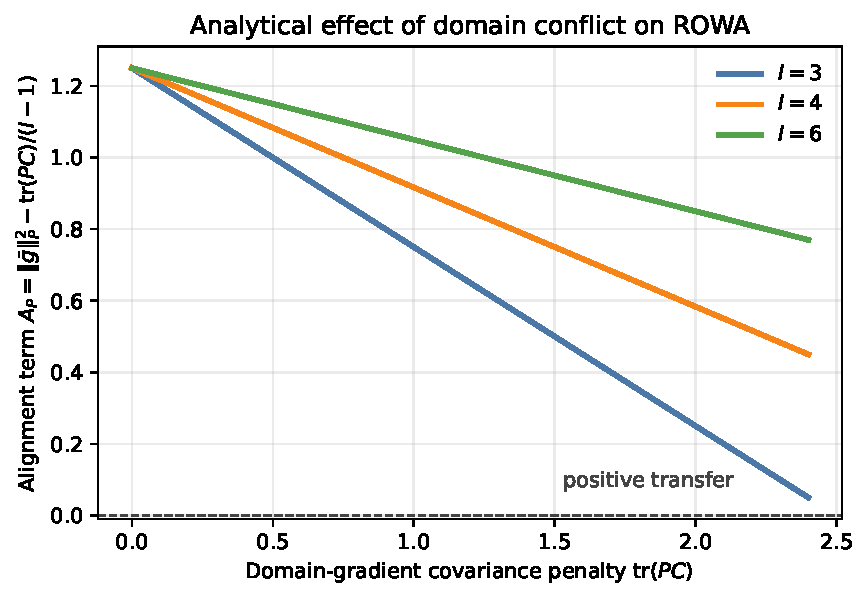
\includegraphics[width=\linewidth]{figures/alignment_covariance_tradeoff.pdf}
    \caption{\textbf{Analytical trade-off implied by Theorem~\ref{thm:decomp}.} For fixed shared descent, domain-gradient covariance linearly reduces the recoverability term. Larger numbers of source domains dilute this penalty by the factor $(I-1)^{-1}$.}
    \label{fig:tradeoff}
\end{figure}

\subsection{Why pooled flatness is not enough}

Theorem~\ref{thm:decomp} already suggests what pooled-flatness criteria miss: domain-gradient covariance. The next theorem makes this failure mode explicit.

\begin{theorem}[Constructive separation from pooled-flatness selectors]
\label{thm:separation}
Fix $I=2$, $P=I$, and $\beta > 0$. Let $u,v \in \RR^p$ be nonzero vectors with $u^\top v = 0$. Consider two local two-domain families around the same checkpoint $\theta$:
\begin{align}
    L_1^{A}(\theta+\Delta) &= \ell_0 + u^\top \Delta + \frac{\beta}{2}\|\Delta\|^2,\\
    L_2^{A}(\theta+\Delta) &= \ell_0 + u^\top \Delta + \frac{\beta}{2}\|\Delta\|^2,
\end{align}
and
\begin{align}
    L_1^{B}(\theta+\Delta) &= \ell_0 + (u+v)^\top \Delta + \frac{\beta}{2}\|\Delta\|^2,\\
    L_2^{B}(\theta+\Delta) &= \ell_0 + (u-v)^\top \Delta + \frac{\beta}{2}\|\Delta\|^2.
\end{align}
Then the two families satisfy all of the following.
\begin{enumerate}[label=(\roman*), leftmargin=1.5em]
    \item They have the same pooled local loss:
    \begin{equation}
        \frac{1}{2}(L_1^{A}+L_2^{A})(\theta+\Delta) = \frac{1}{2}(L_1^{B}+L_2^{B})(\theta+\Delta)
        = \ell_0 + u^\top \Delta + \frac{\beta}{2}\|\Delta\|^2.
    \end{equation}
    In particular, they have the same pooled gradient and the same pooled Hessian.
    \item Any selector that depends only on pooled loss and pooled flatness statistics is indifferent between the two families.
    \item Their exact \rowa{} core scores at $\theta$ differ strictly:
    \begin{equation}
        R^{\mathrm{ex}}_{B}(\theta;\eta,I)
        =
        R^{\mathrm{ex}}_{A}(\theta;\eta,I)
        +
        \eta \|v\|^2
        +
        \frac{\beta \eta^2}{2}\|v\|^2.
        \label{eq:strict_gap}
    \end{equation}
\end{enumerate}
\end{theorem}

Theorem~\ref{thm:separation} does not say that \rowa{} always beats \swad{}. It says something sharper and safer: there exist DG-relevant local configurations on which any criterion that only sees the pooled loss landscape is provably blind, whereas \rowa{} is not.

\subsection{Dense checkpoint sampling and averaging}

The last two propositions justify the practical structure that \rowa{} inherits from \swad{}: dense checkpoint sampling and window averaging.

\begin{proposition}[Dense checkpoint selection converges to the continuous optimum]
\label{prop:dense}
Let $\theta:[0,T]\to\RR^p$ be a continuous training trajectory and let $s(t) \triangleq S(\theta(t))$ be an $L_s$-Lipschitz score function along the trajectory. Suppose checkpoints are saved at times $0=t_1< t_2 < \cdots < t_K=T$ with maximum gap $\Delta = \max_k (t_{k+1}-t_k)$. Then
\begin{equation}
    \min_{1\le k\le K} s(t_k)
    \le
    \min_{t\in[0,T]} s(t) + \frac{L_s \Delta}{2}.
\end{equation}
Hence the discrete optimum converges to the continuous optimum as $\Delta \to 0$.
\end{proposition}

\begin{proposition}[Window averaging is safe under a local quadratic upper model]
\label{prop:avg}
Suppose a selected window $\{\theta_t\}_{t\in W}$ lies inside a convex neighborhood on which the exact \rowa{} upper bound takes the quadratic form
\begin{equation}
    U(\theta) = c + b^\top \theta + \frac{1}{2}\theta^\top Q \theta,
\end{equation}
with $Q \succeq 0$. Then for any convex weights $\{w_t\}_{t\in W}$,
\begin{equation}
    U\!\left(\sum_{t\in W} w_t \theta_t \right)
    \le
    \sum_{t\in W} w_t U(\theta_t).
\end{equation}
\end{proposition}

Proposition~\ref{prop:avg} is the local convexity statement needed to justify \rowa{}'s final averaging step. It is not a global guarantee for deep networks, but it is the exact local regime in which SWA-style and \swad{}-style averaging are meant to operate.

\section{Experimental Protocol}
\label{sec:experiments}

This section specifies the full intended evaluation. The manuscript is complete in structure, but all \rowa{}-specific quantitative cells remain marked \TBD{} because no experiments have been executed yet.

\subsection{Benchmarks and backbone}

We will evaluate on the five standard DomainBed datasets used by \swad{} and DiWA: PACS \citep{li2017pacs}, VLCS \citep{fang2013vlcs}, OfficeHome \citep{venkateswara2017officehome}, TerraIncognita \citep{beery2018terraincognita}, and DomainNet \citep{peng2019domainnet}. Following prior work \citep{cha2021wad,rame2022diwa,gulrajani2021in}, the primary backbone is ResNet-50 and the primary protocol is leave-one-domain-out evaluation with model selection using held-out source validation domains.

\subsection{Baselines}

We will compare against:
\begin{itemize}[leftmargin=1.4em]
    \item ERM, the DomainBed reference baseline \citep{gulrajani2021in};
    \item CORAL \citep{sun2016coral}, a classical DG baseline and the strongest \swad{} combination reported in \citep{cha2021wad};
    \item SWA \citep{izmailov2018swa};
    \item \swad{} \citep{cha2021wad};
    \item DiWA \citep{rame2022diwa};
    \item training-time one-step DG baselines where available, notably MLDG \citep{li2018mldg};
    \item optional auxiliary analyses against SAM \citep{foret2021}.
\end{itemize}

\subsection{\rowa{} variants}

We plan to report the following variants:
\begin{itemize}[leftmargin=1.4em]
    \item \textbf{\rowa-FO}: first-order score, identity preconditioner;
    \item \textbf{\rowa-Exact}: exact one-step score, identity preconditioner;
    \item \textbf{\rowa-Exact-Diag}: exact one-step score with diagonal preconditioner;
    \item \textbf{\rowa-Single}: best single checkpoint without window averaging;
    \item \textbf{\rowa-Window}: low-score window averaging as the default method.
\end{itemize}

The main hyperparameters are the transfer step size $\eta$, gap weight $\lambda$, and window width $\delta$. The primary sweep will use a logarithmic grid over $\eta$, a small grid over $\lambda \in \{0, 0.1, 0.3, 1.0\}$, and a small set of normalized sublevel widths for $\delta$.

\subsection{Metrics}

We will report:
\begin{itemize}[leftmargin=1.4em]
    \item mean \ood{} accuracy;
    \item mean \iid{} accuracy on held-out source validation domains;
    \item worst-domain \ood{} accuracy;
    \item correlation between checkpoint score and final \ood{} accuracy;
    \item added compute relative to \swad{}.
\end{itemize}

\begin{figure}[t]
    \centering
    
\includegraphics[width=\linewidth]{figures/dense_window_schematic.pdf}
    \caption{\textbf{Dense checkpoint sampling and sublevel-window averaging.} \rowa{} uses the same practical scaffold that made \swad{} attractive: dense checkpointing plus averaging over a contiguous region around the best score. The figure is schematic, not empirical.}
    \label{fig:window}
\end{figure}

\section{Published Reference Results and Placeholder Tables}
\label{sec:results}

We include exact published baselines from prior work so that the quantitative target is clear even before running \rowa{}. All rows for the proposed method remain \TBD{}.

\begin{table*}[t]
    \centering
    \small
    \setlength{\tabcolsep}{5pt}
    \caption{\textbf{Published reference results on DomainBed with ResNet-50.} Numbers are copied from the cited papers and are included here solely as reference targets for the planned \rowa{} evaluation.}
    \label{tab:published}
    \begin{tabular}{lcccccc}
        \toprule
        Method & PACS & VLCS & OfficeHome & TerraInc & DomainNet & Avg \\
        \midrule
        ERM \citep{cha2021wad,rame2022diwa} & 85.5 & 77.5 & 66.5 & 46.1 & 40.9 & 63.3 \\
        CORAL \citep{rame2022diwa} & 86.2 & 78.8 & 68.7 & 47.6 & 41.5 & 64.6 \\
        \swad{} \citep{cha2021wad} & 88.1 & 79.1 & 70.6 & 50.0 & 46.5 & 66.9 \\
        CORAL + \swad{} \citep{cha2021wad} & 88.3 & 78.9 & 71.3 & 51.0 & 46.8 & 67.3 \\
        DiWA (random init, $M=60$) \citep{rame2022diwa} & 89.0 & 79.4 & 71.6 & 49.0 & 46.3 & 67.1 \\
        DiWA (LP init, $M=60$) \citep{rame2022diwa} & 89.0 & 78.6 & 72.8 & 51.9 & 47.7 & 68.0 \\
        \midrule
        \rowa{}-FO (ours) & \TBD & \TBD & \TBD & \TBD & \TBD & \TBD \\
        \rowa{}-Exact (ours) & \TBD & \TBD & \TBD & \TBD & \TBD & \TBD \\
        \rowa{}-Exact-Diag (ours) & \TBD & \TBD & \TBD & \TBD & \TBD & \TBD \\
        \bottomrule
    \end{tabular}
\end{table*}

\begin{table*}[t]
    \centering
    \small
    \caption{\textbf{Planned main results table.} Every \rowa{} cell remains intentionally blank pending experiments.}
    \label{tab:main_tbd}
    \begin{tabular}{lcccccc}
        \toprule
        Method & PACS & VLCS & OfficeHome & TerraInc & DomainNet & Avg \\
        \midrule
        \swad{} & 88.1 & 79.1 & 70.6 & 50.0 & 46.5 & 66.9 \\
        DiWA (best published) & 89.0 & 78.6 & 72.8 & 51.9 & 47.7 & 68.0 \\
        \rowa{}-FO & \TBD & \TBD & \TBD & \TBD & \TBD & \TBD \\
        \rowa{}-Exact & \TBD & \TBD & \TBD & \TBD & \TBD & \TBD \\
        \rowa{}-Exact-Diag & \TBD & \TBD & \TBD & \TBD & \TBD & \TBD \\
        \bottomrule
    \end{tabular}
\end{table*}

\begin{table}[t]
    \centering
    \small
    \caption{\textbf{Planned ablations.} These rows are intentionally left as \TBD{}.}
    \label{tab:ablations}
    \begin{tabular}{lc}
        \toprule
        Ablation & Avg \\
        \midrule
        \rowa{}-FO vs. \rowa{}-Exact & \TBD \\
        Identity vs. diagonal preconditioner & \TBD \\
        Single checkpoint vs. low-score window & \TBD \\
        Mean transfer loss only vs. gap-regularized score & \TBD \\
        Score/\ood{} correlation & \TBD \\
        Compute overhead vs. \swad{} & \TBD \\
        \bottomrule
    \end{tabular}
\end{table}

\paragraph{What the theory predicts.}
Although we do not yet report new numbers, the theory makes clear, falsifiable predictions:
\begin{enumerate}[leftmargin=1.4em]
    \item \rowa{} scores should correlate with \ood{} accuracy more strongly than pooled flatness proxies when domain-gradient covariance is non-negligible.
    \item The first-order variant should recover most of the gain if the selected checkpoints are already in a local smooth regime.
    \item Window averaging should outperform single-checkpoint selection whenever the best checkpoints lie inside a locally connected low-score region.
\end{enumerate}

\section{Discussion and Limitations}

\paragraph{What the theory proves.}
The theory proves four concrete facts. First, \rowa{} estimates a DG-relevant population object under environment exchangeability. Second, its exact score admits a clean smoothness upper bound. Third, its first-order term decomposes into shared descent minus domain conflict. Fourth, pooled-flatness selectors provably miss transfer-relevant differences on an explicit class of examples.

\paragraph{What the theory does not prove.}
The theory does not prove universal empirical superiority over \swad{}, DiWA, or any other DG method. It cannot, and claiming otherwise would be irresponsible. The comparison theorems are local and assumption-dependent. Their value is not that they magically solve DG in full generality; it is that they identify a specific failure mode of flatness-only selection and propose a selector that can see it.

\paragraph{Why simplicity still matters.}
\maiwa{} and other posterior-based ideas may be more general, but they are also heavier. If \rowa{} works, it has a realistic path to adoption because its overhead is modest and its implementation footprint is close to \swad{}.

\paragraph{Current practical limitation.}
The most important limitation of this manuscript is obvious: the experiments have not been run. The paper is therefore complete as a research program and theory paper draft, but not yet complete as an empirical claim.

\section{Conclusion}

We proposed \rowa{}, a simple single-run post-hoc DG method based on recoverability rather than pooled flatness. The method scores checkpoints by leave-one-domain-out one-step transfer and averages a contiguous low-score window. Our analysis shows that \rowa{} directly targets a DG-relevant object, decomposes into shared descent minus domain conflict, and distinguishes examples that flatness-only selectors cannot. The full empirical section remains to be filled in, but the paper now contains the method, the theory, the protocol, the reference baselines, and the assets needed to execute that evaluation.

\bibliographystyle{unsrtnat}
\bibliography{references}

\appendix

\section{Detailed Proofs}

\subsection{Proof of Proposition~\ref{prop:unbiased}}

\begin{proof}
Define
\begin{equation}
    h(E_1,\dots,E_I)
    \triangleq
    \frac{1}{I}\sum_{i=1}^{I}
    L_{E_i}\left(
    \theta - \eta P \frac{1}{I-1}\sum_{j\neq i}\nabla L_{E_j}(\theta)
    \right).
\end{equation}
Because $(E_1,\dots,E_I)$ are \iid{}, the joint law is exchangeable. Therefore every summand in $h$ has the same expectation:
\begin{align}
    \EE[h(E_1,\dots,E_I)]
    &=
    \frac{1}{I}\sum_{i=1}^{I}
    \EE\left[
    L_{E_i}\left(
    \theta - \eta P \frac{1}{I-1}\sum_{j\neq i}\nabla L_{E_j}(\theta)
    \right)
    \right] \\
    &=
    \EE\left[
    L_{E_1}\left(
    \theta - \eta P \frac{1}{I-1}\sum_{j=2}^{I}\nabla L_{E_j}(\theta)
    \right)
    \right].
\end{align}
Renaming $E_1$ as $E_0$ and $(E_2,\dots,E_I)$ as $(E_1,\dots,E_{I-1})$ yields
\begin{equation}
    \EE[h(E_1,\dots,E_I)] = \mathcal{R}_{\rho}(\theta;\eta,P).
\end{equation}
Since $h = \widehat{\mathcal{R}}_I(\theta;\eta,P)$ by definition, the claim follows.
\end{proof}

\subsection{Proof of Theorem~\ref{thm:smooth}}

\begin{proof}
Fix a domain $i$. By Assumption~\ref{ass:smooth}, for any $\Delta$,
\begin{equation}
    L_i(\theta+\Delta)
    \le
    L_i(\theta) + \langle g_i(\theta), \Delta\rangle + \frac{\beta}{2}\|\Delta\|^2.
\end{equation}
Substitute $\Delta = -\eta P g_{-i}(\theta)$:
\begin{align}
    L_i(\theta - \eta P g_{-i}(\theta))
    &\le
    L_i(\theta)
    -
    \eta \langle g_i(\theta), P g_{-i}(\theta)\rangle
    +
    \frac{\beta \eta^2}{2}\|P g_{-i}(\theta)\|^2.
\end{align}
Average over $i=1,\dots,I$:
\begin{align}
    \frac{1}{I}\sum_{i=1}^{I}L_i(\theta - \eta P g_{-i}(\theta))
    &\le
    \frac{1}{I}\sum_{i=1}^{I}L_i(\theta)
    -
    \eta\frac{1}{I}\sum_{i=1}^{I}\langle g_i(\theta), P g_{-i}(\theta)\rangle \nonumber\\
    &\quad
    +
    \frac{\beta \eta^2}{2}\frac{1}{I}\sum_{i=1}^{I}\|P g_{-i}(\theta)\|^2.
\end{align}
Recognizing the definitions of $\bar L(\theta)$, $A_P(\theta)$, and $B_P(\theta)$ proves
\begin{equation}
    R^{\mathrm{ex}}(\theta;\eta,P)
    \le
    \bar L(\theta) - \eta A_P(\theta) + \frac{\beta \eta^2}{2}B_P(\theta).
\end{equation}
\end{proof}

\subsection{Proof of Corollary~\ref{cor:improve}}

\begin{proof}
Theorem~\ref{thm:smooth} gives
\begin{equation}
    R^{\mathrm{ex}}(\theta;\eta,P)
    \le
    \bar L(\theta) - \eta A_P(\theta) + \frac{\beta\eta^2}{2}B_P(\theta).
\end{equation}
If $A_P(\theta) > \frac{\beta\eta}{2}B_P(\theta)$, then
\begin{equation}
    -\eta A_P(\theta) + \frac{\beta\eta^2}{2}B_P(\theta) < 0.
\end{equation}
Therefore
\begin{equation}
    R^{\mathrm{ex}}(\theta;\eta,P) < \bar L(\theta).
\end{equation}
\end{proof}

\subsection{Proof of Theorem~\ref{thm:decomp}}

\begin{proof}
We first derive Eq.~\eqref{eq:alignment_decomp}. By definition,
\begin{equation}
    g_{-i} = \frac{1}{I-1}\sum_{j\neq i} g_j
    = \frac{I\bar g - g_i}{I-1}.
\end{equation}
Hence
\begin{align}
    A_P
    &=
    \frac{1}{I}\sum_{i=1}^{I}\left\langle g_i, P\frac{I\bar g - g_i}{I-1}\right\rangle \\
    &=
    \frac{1}{I-1}\left(
        \frac{I}{I}\sum_{i=1}^{I}\langle g_i, P\bar g\rangle
        -
        \frac{1}{I}\sum_{i=1}^{I}\langle g_i, P g_i\rangle
    \right) \\
    &=
    \frac{I}{I-1}\bar g^\top P \bar g
    -
    \frac{1}{I(I-1)}\sum_{i=1}^{I} g_i^\top P g_i.
\end{align}
Expand the second term around $\bar g$:
\begin{align}
    \frac{1}{I}\sum_{i=1}^{I} g_i^\top P g_i
    &=
    \frac{1}{I}\sum_{i=1}^{I}(\bar g + (g_i-\bar g))^\top P(\bar g + (g_i-\bar g)) \\
    &=
    \bar g^\top P \bar g
    +
    \frac{1}{I}\sum_{i=1}^{I}(g_i-\bar g)^\top P(g_i-\bar g),
\end{align}
because $\sum_i (g_i-\bar g)=0$ eliminates the cross terms. Using
\begin{equation}
    \frac{1}{I}\sum_{i=1}^{I}(g_i-\bar g)^\top P(g_i-\bar g)
    =
    \tr\!\left(P C\right),
\end{equation}
we obtain
\begin{align}
    A_P
    &=
    \frac{I}{I-1}\bar g^\top P \bar g
    -
    \frac{1}{I-1}\left(
        \bar g^\top P \bar g + \tr(P C)
    \right) \\
    &=
    \bar g^\top P \bar g - \frac{1}{I-1}\tr(P C).
\end{align}
This proves Eq.~\eqref{eq:alignment_decomp}.

For Eq.~\eqref{eq:curvature_decomp}, note that
\begin{equation}
    g_{-i}
    =
    \bar g - \frac{g_i-\bar g}{I-1}.
\end{equation}
Apply $P$ and square:
\begin{align}
    \|P g_{-i}\|^2
    &=
    \left\|P\bar g - \frac{P(g_i-\bar g)}{I-1}\right\|^2 \\
    &=
    \|P\bar g\|^2
    -
    \frac{2}{I-1}\langle P\bar g, P(g_i-\bar g)\rangle
    +
    \frac{1}{(I-1)^2}\|P(g_i-\bar g)\|^2.
\end{align}
Average over $i$. The middle term vanishes because
\begin{equation}
    \frac{1}{I}\sum_{i=1}^{I} (g_i-\bar g) = 0.
\end{equation}
Therefore
\begin{equation}
    B_P
    =
    \|P\bar g\|^2
    +
    \frac{1}{(I-1)^2}\frac{1}{I}\sum_{i=1}^{I}\|P(g_i-\bar g)\|^2.
\end{equation}
Finally, substitute Eq.~\eqref{eq:alignment_decomp} and Eq.~\eqref{eq:curvature_decomp} into Theorem~\ref{thm:smooth}. This yields Eq.~\eqref{eq:full_decomp}.
\end{proof}

\subsection{Proof of Theorem~\ref{thm:separation}}

\begin{proof}
For family $A$,
\begin{align}
    \frac{1}{2}(L_1^A + L_2^A)(\theta+\Delta)
    &=
    \frac{1}{2}\left(
        \ell_0 + u^\top \Delta + \frac{\beta}{2}\|\Delta\|^2
        +
        \ell_0 + u^\top \Delta + \frac{\beta}{2}\|\Delta\|^2
    \right) \\
    &=
    \ell_0 + u^\top \Delta + \frac{\beta}{2}\|\Delta\|^2.
\end{align}
For family $B$,
\begin{align}
    \frac{1}{2}(L_1^B + L_2^B)(\theta+\Delta)
    &=
    \frac{1}{2}\left(
        \ell_0 + (u+v)^\top \Delta + \frac{\beta}{2}\|\Delta\|^2
        +
        \ell_0 + (u-v)^\top \Delta + \frac{\beta}{2}\|\Delta\|^2
    \right) \\
    &=
    \ell_0 + u^\top \Delta + \frac{\beta}{2}\|\Delta\|^2.
\end{align}
This proves part (i), and part (ii) follows immediately: any selector using only pooled loss and pooled Hessian sees the same local object.

We now compute the \rowa{} score. Since $I=2$, the leave-one-domain-out gradient for each domain is simply the other domain's gradient. At $\Delta=0$, family $A$ has
\begin{equation}
    g_1^A = g_2^A = u.
\end{equation}
Thus
\begin{align}
    R_A^{\mathrm{ex}}(\theta;\eta,I)
    &=
    \frac{1}{2}\left(
        L_1^A(\theta - \eta u) + L_2^A(\theta - \eta u)
    \right) \\
    &=
    \ell_0 - \eta \|u\|^2 + \frac{\beta\eta^2}{2}\|u\|^2.
\end{align}

For family $B$, at $\Delta=0$,
\begin{equation}
    g_1^B = u+v,\qquad g_2^B = u-v.
\end{equation}
Therefore
\begin{align}
    R_B^{\mathrm{ex}}(\theta;\eta,I)
    &=
    \frac{1}{2}\left(
        L_1^B(\theta - \eta(u-v)) + L_2^B(\theta - \eta(u+v))
    \right).
\end{align}
Because $u^\top v = 0$,
\begin{align}
    L_1^B(\theta - \eta(u-v))
    &=
    \ell_0 - \eta (u+v)^\top (u-v) + \frac{\beta\eta^2}{2}\|u-v\|^2 \\
    &=
    \ell_0 - \eta(\|u\|^2 - \|v\|^2) + \frac{\beta\eta^2}{2}(\|u\|^2+\|v\|^2),
\end{align}
and similarly
\begin{align}
    L_2^B(\theta - \eta(u+v))
    &=
    \ell_0 - \eta (u-v)^\top (u+v) + \frac{\beta\eta^2}{2}\|u+v\|^2 \\
    &=
    \ell_0 - \eta(\|u\|^2 - \|v\|^2) + \frac{\beta\eta^2}{2}(\|u\|^2+\|v\|^2).
\end{align}
Hence
\begin{equation}
    R_B^{\mathrm{ex}}(\theta;\eta,I)
    =
    \ell_0 - \eta(\|u\|^2 - \|v\|^2) + \frac{\beta\eta^2}{2}(\|u\|^2+\|v\|^2).
\end{equation}
Subtracting the two expressions gives
\begin{align}
    R_B^{\mathrm{ex}}(\theta;\eta,I) - R_A^{\mathrm{ex}}(\theta;\eta,I)
    &=
    \eta \|v\|^2 + \frac{\beta\eta^2}{2}\|v\|^2 > 0,
\end{align}
which proves Eq.~\eqref{eq:strict_gap}.
\end{proof}

\subsection{Proof of Proposition~\ref{prop:dense}}

\begin{proof}
Let $t^\star \in \argmin_{t\in[0,T]} s(t)$ be a continuous minimizer. Choose a checkpoint index $k$ such that $|t_k - t^\star| \le \Delta/2$; such an index exists by construction of the grid. Since $s$ is $L_s$-Lipschitz,
\begin{equation}
    s(t_k) \le s(t^\star) + L_s |t_k - t^\star| \le s(t^\star) + \frac{L_s \Delta}{2}.
\end{equation}
Taking the minimum over $k$ yields
\begin{equation}
    \min_{1\le k\le K} s(t_k) \le \min_{t\in[0,T]} s(t) + \frac{L_s \Delta}{2}.
\end{equation}
As $\Delta \to 0$, the right-hand side converges to the continuous optimum.
\end{proof}

\subsection{Proof of Proposition~\ref{prop:avg}}

\begin{proof}
Because $Q \succeq 0$, the function $U(\theta)=c+b^\top\theta+\frac{1}{2}\theta^\top Q\theta$ is convex. Convexity implies Jensen's inequality:
\begin{equation}
    U\!\left(\sum_{t\in W} w_t \theta_t\right)
    \le
    \sum_{t\in W} w_t U(\theta_t),
\end{equation}
for any nonnegative weights summing to one. This is exactly the desired claim.
\end{proof}

\section{Additional Implementation Notes}

\paragraph{Identity versus diagonal preconditioning.}
The main paper uses $P_t=I$ for clarity. A diagonal alternative is
\begin{equation}
    P_t = \diag(\hat v_t + \tau)^{-1/2},
\end{equation}
where $\hat v_t$ is either a running second-moment estimate from the optimizer state or a diagonal empirical Fisher on held-out source data. This yields a geometry-aware variant without changing the basic algorithm.

\paragraph{First-order variant.}
The exact variant requires evaluating $L_i(\theta_t - \eta P_t g_{-i,t})$. The first-order variant replaces this with
\begin{equation}
    L_i(\theta_t) - \eta \langle g_{i,t}, P_t g_{-i,t}\rangle.
\end{equation}
The approximation is expected to be accurate when $\eta$ is small and the selected window lies in a smooth neighborhood, which is precisely the regime encouraged by dense checkpointing.

\paragraph{Why a contiguous window?}
The contiguity constraint is inherited from SWA and \swad{}. It is not merely aesthetic. It acts as a cheap surrogate for staying inside one connected low-barrier region, which is the regime in which weight averaging is least likely to jump across incompatible modes.

\end{document}
